

%Cox and Katz (2007) is a study of bias and responsiveness in the 46th through 106th Congresses. Cox and Katz are predominantly concerned with estimating the parameters $\lambda = \{\lambda_t : t = 46, \dots, 106\}$ representing bias in each $C_t$ (Congress t), which they do by maximum likelihood estimation of grouped logit models with linear predictor
%
%$$ \lambda_t + \rho_t \log{\left(\frac{v_t}{1 - v_t} \right)}, $$
%
%\noindent where $\rho$ is responsiveness and $v$ is average Democratic vote share. They use this strategy to estimate what they call ``a sort of running average" of the bias across time, where they take as their estimate of $\lambda_t$ the average estimate of $\lambda$ over the seven congresses centered at $t$, i.e., the set of congresses $\{C_\tau, t-3 \leq \tau \leq t+3\}$. 
%
%Note that this strategy requires using the data for each Congress up to seven times, which can lead to overly precise parameter estimates. Moreover, the estimation strategy used by Cox and Katz treats each of the seven congresses centered at $t$ as providing {\it equal} information about $\lambda_t$, which is unlikely to be the case. 
%
%Many new possibilities are available to us if we can reformulate their model according to the Bayesian approach advocated above. Let $x = \log{\left(\frac{v_t}{1 - v_t} \right)}$. We use the addititive predictor
%
%$$ \eta = f_1(\lambda) + f_2(x),$$
%
%where the $f_j$ are unknown functions such that the vector of evaluations of $f_j$ can be expressed as the product $\theta_j \mathbf{M}_j$ of a parameter vector $\theta_j$ and a design matrix $\mathbf{M}_j$.  We can then assign a prior for $f_j$ by specifying a suitable $\mathbf{M}_j$ and a (typically partially improper) multivariate normal prior 
%%
%$$ p(\theta_j | \tau_j^2) \propto \exp{\left(-\frac{1}{2\tau_j^2} \theta_j^T \mathbf{P}^{-1} \theta_j \right)}, $$
%
%\noindent where we choose to specify a penalty matrix $\mathbf{P}$ that represents our assumptions of temporal dependence between adjacent Congresses. 
%
% For example, suppose we want to specify a prior that reflects a belief that $\partial_t = \{C_{t-2}, C_{t-1}, C_{t+1}, C_{t + 2} \}$ provides information about $C_t$. We will refer to the elements of $\partial_t$ as the {\it neighbors} of $C_t$. We can use an undirected form of a second order random walk or autoregressive prior to penalize deviations from this hypothesized trend, which corresponds to setting $\mathbf{P} = \mathbf{D} - \mathbf{A}$, where $\mathbf{A}$ is a symmetric matrix with $a_{ij} = 1$ if $C_j \in \partial_i$ and 0 otherwise, and $\mathbf{D}$ is a diagonal matrix such that $\forall i = j, \: d_{ij} = \sum_j a_{ij}$.\footnote{It can be useful to conceptualize the neighbor relations as an undirected graph $G$ with vertices $V= \{C_t, t = 46, \dots, 106\}$ and edges connecting the vertices corresponding to neighboring congresses. The penalty matrix $\mathbf{P}$ then has a zero for each missing edge and the resulting multivariate normal distribution is said to form a Markov random field with respect to $G$. The matrices $\mathbf{A}$ and $\mathbf{D}$ are commonly referred to as the adjacency and degree matrices.}   We then specify a hyperprior $p(\tau^2)$, completing the hierarchical model and enabling the concurrent estimation of the unknown function $f$ and the amount of nonparametric smoothing (Fahrmeir and Lang, 2000). 
% 
% Note that this approach enables us to account for temporal dependence without reusing the data to estimate separate a model for each congress. The Bayesian approach advocated here allows the specification of more intricate temporal relationships that better reflect our assumptions of association across time (and across space in other contexts). For example, a second order random walk prior treats $C_{t-1}$ and $C_{t+1}$ as being more informative than $C_{t-2}$ and $C_{t+2}$ about bias in $C_t$, which seems more reasonable. 


\chapter{Empirical example: Cox and Katz (2007)}

To demonstrate the benefits of the methods proposed by \citeA{wawro_designing_2014}, we conduct a reanalysis of \citeA{cox_gerrymandering_2007}, a study of bias and responsiveness in congressional roll-call votes in the 46th through 106th US Congresses. Cox and Katz's findings suggest persistent bias towards the majority party with particularly elevated levels during the periods from 1889-1910 and 1961-2000, known as the period of ``czar rule" and the post-packing era, respectively. Analyzing the data using Bayesian STAR models we find much weaker evidence for bias towards the majority over the time periods in question. 

\section{Definitions}


\paragraph{Bias}
In the legislative context of Cox and Katz's analysis, bias is defined as an advantage for one party in the efficiency with which its votes translate into legislative victories. For example, consider a majority party with only a small advantage in the number of seats its members occupy. If the majority is well-organized and unified it may win a much larger proportion of votes than its slim seat advantage would typically suggest. 

\paragraph{Responsiveness} MISSING DEFINITION


\section{Data}

The data include -- with a few exceptions detailed below -- all roll-call votes in the U.S. House of Representatives during the 46th through 106th Congresses, corresponding to the period from 1879 to 2001.  Following Cox and Katz, excluded from the analysis are any records that meet at least one of the following three conditions:

\begin{itemize}
\singlespacing
\item The majority of both parties voted for the same position 
\item The purpose of the vote was electing the Speaker of the House
\item The vote required a two-thirds majority for passage.
\end{itemize}

The resulting data consist only of votes that required a simple majority for passage and on which the Republican and Democratic parties were in clear opposition. 

Let $RC_{it}$ denote the result of roll-call vote $i$ in Congress $t$ such that 

{\singlespacing
$$ RC_{it} =
\begin{cases} 
1, & \text{ if Democratic position wins vote $i$ in Congress $t$} \\
0, & \text{ if Republican position wins vote $i$ in Congress $t$.}
\end{cases}
$$
}
%
Here, the Democratic position refers to the outcome preferred by the majority of Democrats.  The definition is analogous for the Republican position.

The outcomes of interest are the number of wins ($w_t^{DEM}$) and proportion of wins ($p_t^{DEM}$) for the Democratic position in each Congress $t$

$$ w_t^{DEM} = \sum_{i=1}^{n_t} RC_{it}, \qquad p_t^{DEM} = w_t^{DEM} / n_t.\footnote{The superscript {\it MAJ} (e.g. $w_t^{MAJ}$) will be used later in the thesis as a general way of referring to the majority party in a specific time period. While the data is organized and more naturally described in terms of $w_t^{DEM}$ and $w_t^{REP}$ (which is just $n_t-w_t^{DEM}$), the proposed statistical model is more straightforward to implement in terms of $w_t^{MAJ.}$}$$

Here $n_t$ is the number of roll-call votes in Congress $t$, which ranges from a minimum of 33 votes in the 70th Congress (1927-1929) to a maximum of 836 votes in the 104th Congress (1995-1997). The median number is 143 votes.  

The sole predictor of interest is $v^{RATIO}$, the ratio of the average vote share earned by the Democratic position to the average vote share earned by the Republican position in each Congress.  For each Congress the average is taken over all roll-call votes.  For vote $i$ in Congress $t$, let $\pi_{it}^{DEM}$ be the proportion of representatives who cast their vote in favor of the Democratic position.  Then the mean vote shares for the Democratic and Republican positions in Congress t is

{\singlespacing
$$v_t^{DEM} = \frac{1}{n_t} \sum_{i=1}^{n_t} \pi_{it}^{DEM}, \qquad v_t^{REP} = 1 - v_t^{DEM}$$
}
%
\noindent and the ratio of Democratic to Republican vote shares is simply $v_t^{RATIO} = v_t^{DEM} / v_t^{REP}$. Figure~\ref{fig:log_vratio_vs_ptdem} shows $\log{(v^{RATIO} )}$ plotted against $p^{DEM}$. The shape of the curve is similar to the standard seats-votes curve used in analyses of bias and responsiveness in electoral contexts. The curve is analogous in the legislative context of Cox and Katz's example, although we are not concerned with seat shares in a given Congress but rather roll-call vote shares ($p_t^{DEM}$ and $p_t^{REP}$). This is discussed further in the Methods section. 

The trends of $\log{(v^{RATIO} )}$ and $p^{DEM}$ over time are shown in the visual summary of the data set in Figure~\ref{fig:data_summary}.

%FIGURE
\begin{figure}
\centering
	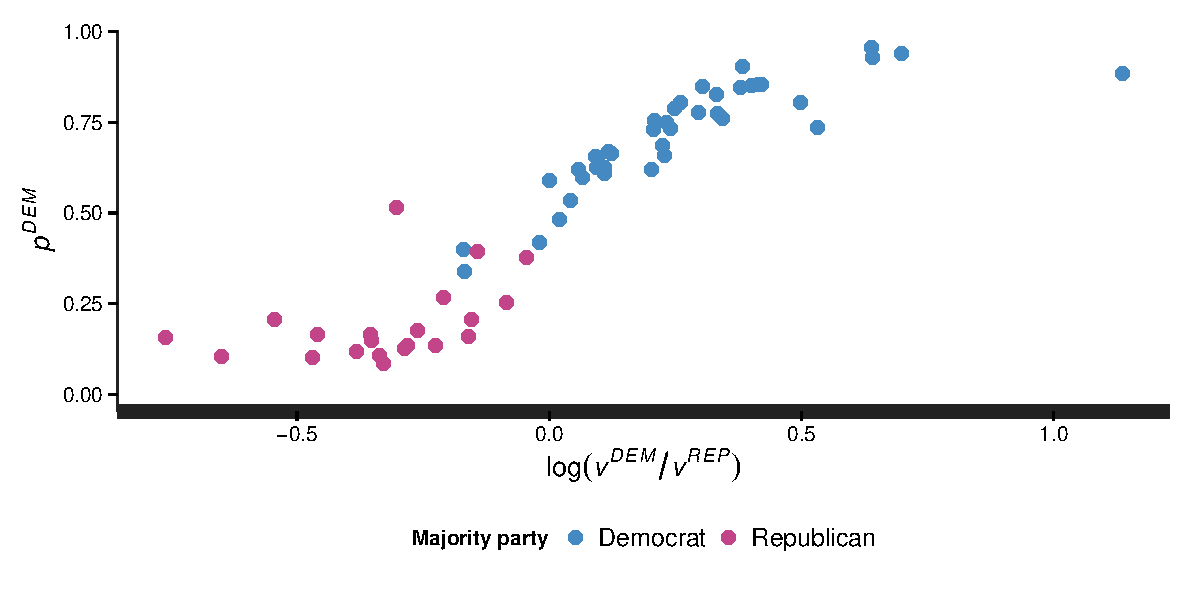
\includegraphics[scale=0.75]{sections/figs/logvratio_vs_pdem}
\caption{$\log{(v^{RATIO} )}$  vs. $p^{DEM}$}
\label{fig:log_vratio_vs_ptdem}
\end{figure}
%



%FIGURE
\begin{figure}
\centering
	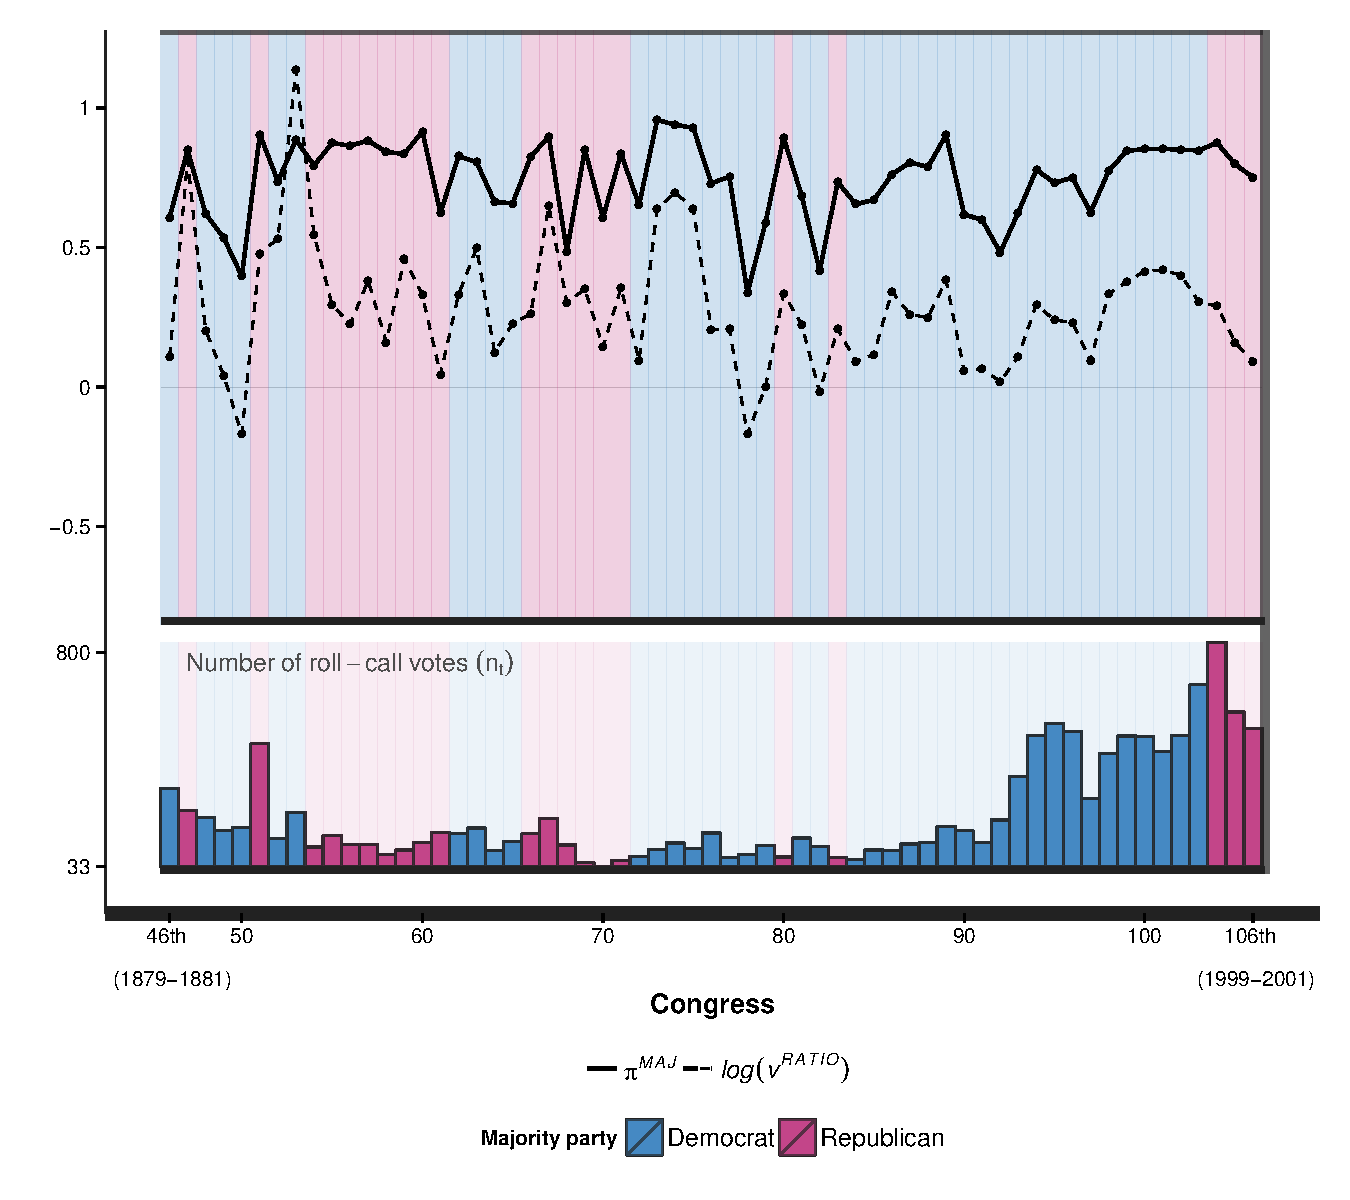
\includegraphics[scale=0.75]{sections/figs/vis_summary}
\caption{Visual summary of the data}
\label{fig:data_summary}
\end{figure}
%

One method of identifying bias toward or against the majority party is to estimate $E[p_t^{MAJ} |v_t^{MAJ}=0.5]$, the proportion of majority party victories conditional on equal vote share, and compare the estimate to $0.5$, the expected proportion of majority party victories in the absence of bias.  There are many close votes in the data -- that is, votes where $v_t^{MAJ} \approx 0$ -- which can be used to estimate $E[p_t^{MAJ} |v_t^{MAJ}=0.5]$.  Figure 2, below, shows the proportion of majority party victories under four different definitions of a close votes corresponding to margins of victory of 0.125\%, 0.25\%, 0.5\%, and 1.0\%. 

\vskip1cm
FIGURE
\vskip1cm

\section{Methods of Analysis}
\subsection{Methods}
\label{subsection_methods}

One of the analyses conducted by Cox and Katz concerns the estimation of parameters  $\lambda = (\lambda_t : t = 46, \dots, 106)$ representing bias (on the logit scale) toward the majority party in each $C_t$ (Congress $t$), which is done by maximum likelihood estimation of grouped logit models with linear predictor

{\singlespacing
$$ \lambda_t + \rho_t \log{\left(v_t^{RATIO} \right)}. $$
}
%
Here the parameter $\rho$ represents responsiveness, as defined above. The estimation of $\lambda$ and $\rho$ by grouped logit models follows naturally from solving the seats-votes equation for the average seat share, which in the legislative context of Cox and Katz's example is $p^{DEM}$, the expected roll-call win share for the Democrats 

{\singlespacing
$$  
  E(p^{DEM}_t)  = \left(1 + \exp{\left\{- \lambda_t - \rho_t \log{\left( v_t^{RATIO}  \right)}\right\}}\right)^{-1},
$$
}
%
\noindent which is the familiar logistic function. 

Cox and Katz's strategy is to estimate what they call ``a sort of running average" of bias across time (p. 116). To do this they take as their estimate of $\lambda_t$ the average estimate of $\lambda$ over the seven congresses centered at $t$, the set $\{C_\tau, t-3 \leq \tau \leq t+3\}$. The authors attempt to account for temporal dependence in $\lambda$ but their approach requires reusing the data to estimate models for each Congress and the observations for each Congress are used up to seven times.  \citeA{goodrich_designing_2012} point out that recycling data in this fashion can lead to overly precise parameter estimates. 

Although Cox and Katz do not acknowledge this potential for exaggerated precision, they do call attention to another important concern. To obtain reasonable estimates, their method requires a nontrivial amount of variation in average vote share ($v^{RATIO}$) between the seven Congresses that comprise each set $C_\tau$. 

The analysis proposed in thesis overcomes both of these concerns by employing a hierarchical Bayesian framework with partial pooling. Following Cox and Katz, a BetaBinomial likelihood is used, however the linear predictor is replaced by the structured additive predictor $\eta$. The data model with logit link function is 

$$w_t^{MAJ} | n_t, \alpha_t, \beta_t \sim {\rm BetaBinomial}(n_t, \alpha_t, \beta_t),$$
$$ \alpha_t = \theta_t \phi, \qquad \beta_t = \theta_t (1 - \phi),$$
$$ \log\left({\frac{\theta_t}{1 - \theta_t}}\right) = \eta_t = f_{\lambda}(\lambda_t) + f_\rho \left(\log{(v_t^{RATIO})}\right).$$

The ${\rm BetaBinomial}(\alpha,\beta)$ distribution can be thought of as a compound distribution resulting from a binomial distribution where the probability parameter follows a ${\rm Beta}(\alpha,\beta)$ distribution. In other words, rather than assuming that the Congress-by-Congress probabilities of a majority party roll-call victory are independent and identically distributed -- in which case the binomial distribution would suffice -- the BetaBinomial  allows for direct modeling of the variation in the probability of victory through the Beta distribution. The parameters $\alpha$ and $\beta$ govern the shape of the Beta distribution, however it is both more intuitive and computationally attractive to reparameterize in terms of the mean $\theta$, which requires introducing a parameter $\phi$ as the sum of $\alpha$ and $\beta$.  This parameterization allows for ${\rm logit}(\theta)$ to be estimated by the semi-parametric structured additive predictor $\eta$ of the STAR model. 

Instead of Cox and Katz's ``sort of running average" approach, the hierarchical Bayesian STAR model entails estimating the unknown functions $f_\lambda$ and $f_\rho$. As we've seen, the vector of evaluations of the unknown functions can be conveniently expressed as the products 

{\singlespacing
$$
\mathbf{f}^{eval}_\lambda = \lambda \mathbf{M}_\lambda, 
\qquad 
\mathbf{f}^{eval}_\rho = \rho \mathbf{M}_\rho, 
$$
}
%
\noindent of the parameter vectors $\lambda$ and $\rho$ of length 61 (the number of Congresses in the data) and  $N \times 61$ design matrices  $\mathbf{M}_\lambda$ and  $\mathbf{M}_\rho$ (where $N$ is the total number of observations in the data).   

The the structured additive predictor $\eta$ can be written compactly in vector notation as 

{\singlespacing
$$ \eta = f_\lambda(\lambda) +  f_\rho(\log{(v^{RATIO})}) = \lambda \mathbf{M}_\lambda + \rho \mathbf{M}_\rho.$$
}
%
The matrices $\mathbf{M}_\lambda$ and $\mathbf{M}_\rho$ are identical in structure but not content. Since $\lambda$ plays the role of an intercept -- that is, the parameters in $\lambda$ are not coefficients -- the elements of $\mathbf{M}_\lambda$ are zeros and ones indicating the Congress to which each observation pertains. For $\mathbf{M}_\rho$ each element is either a zero or the appropriate value of $\log{(v^{RATIO})}$. 

% Discuss challenges with sparse matrices? Either here or in the lit review section

The GMRF priors for $f_{\lambda}$ and $f_{\rho}$ are expressed as prior distributions for the parameter vectors $\lambda$ and $\rho$ as 

{\singlespacing
$$ 
p(\lambda | \tau_\lambda^2) \propto \exp{\left(-\frac{1}{2\tau_\lambda^2} \: \lambda' \, \mathbf{P}  \, \lambda \right)}, 
\qquad
p(\rho | \tau_\rho^2) \propto \exp{\left(-\frac{1}{2\tau_\rho^2} \: \rho' \, \mathbf{P} \, \rho \right)}
 $$
}
%
\noindent where the penalty matrix $\mathbf{P}$ encodes assumptions about the temporal dependence between Congresses.\footnote{The impropriety of this prior stems from the fact that the matrix  $\mathbf{P}$ is not full rank.  The computational challenges this presents can be overcome by coding the model in a statistically equivalent but less intuitive form.} To model temporal dependence such that the set of Congresses $\partial_t = \{C_{t-2}, C_{t-1}, C_{t+1}, C_{t + 2} \}$ provides information about $C_t$, the undirected $RW_2$ prior discussed earlier is used to penalize deviations from this hypothesized trend. This corresponds to constructing $\mathbf{P}$ from the adjacency matrix $\mathbf{A}$ with $a_{ij} = 1$ if $C_j \in \partial_i$ and 0 otherwise.


%As alluded to above, modeling the temporal dependence between Congresses is accomplished via the choice of penalty matrix $\mathbf{P}$. To model temporal dependence such that the set of Congresses $\partial_t = \{C_{t-2}, C_{t-1}, C_{t+1}, C_{t + 2} \}$ provides information about $C_t$, an undirected form of a second order random walk or autoregressive prior is used to penalize deviations from this hypothesized trend. This corresponds to setting $\mathbf{P} = \mathbf{D} - \mathbf{A}$, where $\mathbf{A}$ is a symmetric matrix with $a_{ij} = 1$ if $C_j \in \partial_i$ and 0 otherwise, and $\mathbf{D}$ is a diagonal matrix such that $\forall i = j, \: d_{ij} = \sum_j a_{ij}$. It can be useful to conceptualize the neighbor relations described by each set $\partial_t$ as an undirected graph $G$ with vertices $V=\{C_t: t=46,\dots,106\}$ and edges connecting the vertices corresponding to neighboring Congresses.\footnote{Note that here the term ``neighbor" is not reserved only for adjacent Congresses, but rather any Congress in $\partial_t$ is considered a neighbor of Congress $t$.} The penalty matrix $\mathbf{P}$ then has a zero for each missing edge and the resulting multivariate normal distribution is a GMRF with respect to $G$.
%
%The matrices $\mathbf{A}$ and $\mathbf{D}$ are commonly referred to as the adjacency and degree matrices because encoded in $\mathbf{A}$ are all neighbor relationships (in this case a temporal relationship between Congresses) and the diagonal elements of $\mathbf{D}$ are the number of neighbors (the degree) of each vertex.
%
%To illustrate why this form of $\mathbf{P}$ captures these particular assumptions, consider $N$ measurements of a variable $x$, with each measurement made at one of $T$ evenly spaced points in time. For simplicity assume $N=T$ and that unit of $x$ is a unit of time.  The sequence of equally spaced time measurements $(x^{[t]})_{t=1}^T$ corresponds to a grid of points on a line.  Fahrmeir & Lang (2001) suggest several possible choices for a prior on a smooth function $f(x)$, the simplest of which is a first order random walk ($RW_1$) prior.  Under the $RW_1$ prior, the first differences
%
%$$\Delta_t = f(x^{[t]}) - f(x^{[t-1]})$$
%
%are treated as independent and identically distributed standard normal random variables. 
%
%While this formulation of the $RW_1$ prior is {\it directed}, conditioning also on $f(x^{[t+1]})$ -- one step into the future -- forms an undirected $RW_1$, where the neighbors of time $t$ are both $t-1$ and $t+1$.  The associated graph $G$ therefore has vertices $V=\{v_t : t=1,\dots,T\}$, each of which has two neighbors, with the exception of $v_1$ and $v_T$, which have one neighbor. The penalty matrix $\mathbf{P}$ corresponding to the $RW_1$ prior with equally with equally spaced observations is the tridiagonal matrix
%
%$$ \mathbf{P} = \mathbf{D} - \mathbf{A} =  \begin{bmatrix}
%1  	& -1 	& 		& 	& \\
%-1  	& 2 	& -1 		& 	& \\
%  	& -1 	& \ddots 	& \ddots	& \\
%  	&  	& \ddots 	& 2 	& -1\\
%  	&  	& 		& -1 	& 1\\
%\end{bmatrix}
%.
%$$
%
%The $RW_2$ prior used in this thesis is simply an extension of the $RW_1$ to the case where, in addition to $x^{[t-1]}$  and $x^{[t+1]}$, the measurements $x^{[t-2]}$  and $x^{[t+2]}$ are also considered neighbors of $x^{[t]}$. The construction of $\mathbf{P}$ as the matrix difference $\mathbf{D} - \mathbf{A}$ also allows the estimation of an optional scalar parameter $\gamma \in [0,1]$, which, as a coefficient on $\mathbf{A}$, can be interpreted as representing the strength of dependence (Rue and Held, 2005).\footnote{The resulting precision matrix $\mathbf{Q}= (\mathbf{D}- \gamma \mathbf{A})/\tau^2$ is the defining feature of the conditional autoregressive (CAR) model.  When $\gamma$ is fixed at 1, and thus $\mathbf{P}= \mathbf{D} - \mathbf{A}$, it is known as the intrinsic conditional autoregressive (ICAR) model.} In the results section it will be demonstrated that the degree to which the proposed model fits the data depends (slightly but non-negligibly) on the inclusion of $\gamma$. 



\subsection{Estimation}

For notational convenience, let $y$ denote the outcome $w^{MAJ}$ and $X$ denote the observed data $n$ and $v^{RATIO}$. We require the joint posterior distribution

{\singlespacing
\begin{align*}
p(\lambda, \rho, \tau^2_\lambda, \tau^2_\rho, \phi | y, X) & \propto p(\lambda, \rho, \tau^2_\lambda, \tau^2_\rho, \phi) p(y | \lambda, \rho, \tau^2_\lambda, \tau^2_\rho, \phi,  X)  \\
& = p(\phi) p(\tau^2_\lambda) p(\tau^2_\rho)  p(\lambda | \tau^2_\lambda) p(\rho | \tau^2_\rho) \prod_i p(y_i | \eta_i, X_i) 
\end{align*}
}
%
\noindent where the second line follows from assumptions conditional independence.\footnote{In particular we assume that hyperparameters are mutually independent in their priors, $p(\lambda | \tau^2_\lambda)$ and $p(\rho | \tau^2_\rho)$ are conditionally independent, and the observations $y_i$ are independent conditional on parameters and predictors.}\footnote{The absence of the previously mentioned parameters $\alpha$, $\beta$, and $\theta$ from the expression for the posterior distribution is due to the fact that their values are determined by the other parameters.} 

Estimation is performed numerically by Markov chain Monte Carlo (MCMC) methods and implemented via RStan, the R interface to the probabilistic programming language and C++ library Stan \shortcite{rstan_software:2015}.\footnote{All relevant R and Stan code will be made publicly available in a repository on GitHub.} Since this is the first attempt to estimate these models in Stan that we are aware of, the next section is a description of the estimation strategy and the code required to carry it out in Stan.


\subsection{Stan} 

Stan is a probabilistic modeling language, MCMC sampler, and optimizer. The particular MCMC algorithm implemented in Stan is a variant of Hamiltonian Monte Carlo (HMC) called the no-U-turn sampler (NUTS) \shortcite{hoffman_2012}. Borrowing from physics the concepts and mathematics behind Hamiltonian dynamics, HMC treats the vector of unknown parameters as the position of a particle. In Hamiltonian dynamics, momentum and position change continuously over time, with the gradient of the particle's potential energy function --  which corresponds to the negative log posterior -- responsible for changes in momentum and momentum governing changes in position. Stan works by simulating a discretization of this process, making necessary corrections to preserve detailed balance (i.e., to ensure that the resulting Markov chains are reversible). 

Several characteristics of HMC, and in particular Stan's implementation of HMC, make it a more appealing choice than traditional Metropolis-Hastings (M-H) and Gibbs samplers in many cases. Both M-H and Gibbs samplers suffer from random walk behavior that leads to inefficient exploration of the parameter space. Using gradient information, HMC can find posterior modes much more efficiently, greatly reducing the number of iterations required to obtain a sufficient number of effective draws from the posterior. 

M-H samplers in particular also require a great deal of tuning from the user. Although HMC itself does not overcome this problem, Stan's automatically takes care of the tuning during a warmup period before sampling. Gibbs sampling has an advantage over MH in that it does not require tuning, but a serious drawback is that Gibbs sampling requires the full conditional distributions of all parameters. Except in a limited number of cases, full conditionals are difficult or impossible to derive, which results in a small number of prior distributions that are feasible to use with Gibbs samplers. In particular, conjugate priors are often used even when more believable priors are available. On the other hand, there is no advantage to conjugacy when using Stan. Users are free to specify priors that more accurately reflect their prior knowledge. 

For a more thorough introduction to Stan see \citeA{stan_development_team_stan_2015} and \citeA{gelman_bayesian_2013}. 

\subsubsection{Data}

In the {\tt data} block of a Stan model we declare the data that will be passed to Stan, in this case from R. The {\tt transformed data} block contains transformations of the variables declared in the {\tt data} block. The declarations below are all straightforward, except for the matrix {\tt P\_inv}. This is the inverse of the difference of the degree and adjacency matrices, which is precomputed and passed to Stan as data. In {\tt transformed data} we compute the Cholesky decomposition of {\tt Pinverse}, which will be used for a more efficient implementation of the multivariate normal distributions required for the GMRF priors. Values for the location and scale parameters of the Cauchy distribution are also set in {\tt transformed data}. 


\begin{singlespacing}
\small 
\begin{verbatim}
data {
  // dimensions
  int<lower=1>              N ; # number of observations
  int<lower=1>              C ; # number of congresses (time periods)

  // variables
  int<lower=1,upper=C>      cong[N] ;   # maps between observations & congresses
  int<lower=1,upper=56>     nVotes[N] ; # numerber of votes
  int<lower=0,upper=55>     nWins[N] ;  # number of majority party victories
  real                      vRatio[N] ; # vRatio

  // inverse of penalty matrix for GMRF prior
  matrix[C,C]               Pinverse ;
}
transformed data {
  real<lower=0> tau_scale ;   # scale for Cauchy priors on taus
  real<lower=0> tau_loc ;     # location for Cauchy priors on taus
  matrix[C,C] cholPinverse ;  # Cholesky decomposition of Pinverse

  tau_loc <- 0.0 ;
  tau_scale <- 2.5 ;
  cholPinverse <- cholesky_decompose(Pinverse) ;
}
\end{verbatim}
\end{singlespacing}


\subsubsection{Parameters}

In the {\tt parameters} and {\tt transformed parameters} blocks we declare model parameters and deterministic transformations of the declared parameters. 

\begin{singlespacing}
\small
\begin{verbatim}
parameters {
  real<lower=0>         phi ;
  vector[C]             bias_noise ;
  vector[C]             resp_noise ;
  real<lower=0>         tau_sq_bias_noise ;
  real<lower=0>         tau_sq_resp_noise ;
}
\end{verbatim}
\end{singlespacing}


\noindent Parameter names with the suffix ${\tt \_noise}$ denote variables to be given standard normal priors. Stan tends to work best if the target posterior distribution is marginally standard normal and uncorrelated and parameters on a  similar scale. This means that it can help improve efficiency and convergence if variables defined in {\tt parameters} are given standard normal priors when possible and then transformed in {\tt transformed parameters} to have the desired distribution.\footnote{This is an extremely oversimplified description and a thorough examination of this issue is beyond the scope of this thesis. See \citeA{betancourt_hamiltonian_2013}.} 

In the {\tt transformed parameters} block below both ${\tt tau\_sq\_noise}$ parameters are transformed using the inverse-CDF method such that ${\tt tau\_sq\_bias}$ and ${\tt tau\_sq\_resp}$ have half-Cauchy distributions.\footnote{The inverse-CDF of the Cauchy distribution with location $\ell$ and scale $s$ is $F^{-1}(p, \ell,s)  = \ell + s \tan{\{ \pi (p - 0.5)\}}$. Thus if $z \sim \mathcal{N}(0,1)$ with CDF $\Phi$ then $\ell + s \tan{\{ \pi (\Phi(z) - 0.5)\}}$ is distributed Cauchy$(\ell, s)$. The transformations above therefore result in half-Cauchy$({\tt tau\_loc}, {\tt tau\_scale})$ distributions due to the constraints that ${\tt tau\_sq_bias\_noise}$ and ${\tt tau\_sq\_resp\_noise}$ be positive.} \citeA{gelman_prior_2006} recommends the half-Cauchy as a good default choice for a weakly informative prior on scale parameters.\footnote{The Cauchy prior can be considered weakly informative in that, while most of the mass is concentrated near the median, the tails are fat enough to allow for considerable variation. In fact, the variance of a Cauchy distribution is infinite.}

The transformations of {\tt bias\_noise} and {\tt resp\_noise} lead to the multivariate normal distributions required for the GMRF priors. 

\begin{singlespacing}
\small
\begin{verbatim}
transformed parameters {
  vector[C]             b_bias ;
  vector[C]             b_resp ;
  real<lower=0>         tau_bias ;
  real<lower=0>         tau_resp ;

  tau_sq_bias <- tau_loc + tau_scale * tan(pi() * (Phi_approx(tau_sq_bias_noise) - 0.5)) ;
  tau_sq_resp <- tau_loc + tau_scale * tan(pi() * (Phi_approx(tau_sq_resp_noise) - 0.5)) ;

  b_bias  <- (tau_sq_bias * cholPinverse) * bias_noise ;
  b_resp  <- (tau_sq_resp * cholPinverse) * resp_noise ;
}
\end{verbatim}
\end{singlespacing}

\noindent The lines
%
\begin{singlespacing}
\small
\begin{verbatim}
b_bias  <- (tau_sq_bias * cholPinverse) * bias_noise ; 
b_resp  <- (tau_sq_resp * cholPinverse) * resp_noise ; 
\end{verbatim}
\end{singlespacing}

\noindent come from the fact that if $z$ is a $K$-vector of iid standard normal random variables $z_k \sim \mathcal{N}(0,1)$ and $\theta = \mu + L z$, where $LL' = \boldsymbol{\Sigma}$, then $\theta \sim \mathcal{N}_K (\mu, \boldsymbol{\Sigma})$. This is analogous to the univariate case where $\theta = \mu + \sigma z$ and $z \sim \mathcal{N}(0,1)$ implies that $\theta \sim \mathcal{N}(\mu, \sigma^2)$. The advantage to this approach is twofold. For one, directly specifying a multivariate normal distribution for $\theta$ would require repeated computation of the inverse matrix $\Sigma^{-1}$. Additionally, unlike the elements of $\theta$, the elements of $z$ are independent which can lead to large gains in efficiency for MCMC algorithms in terms of effective sample size \shortcite{stan_development_team_stan_2015}. 

\subsubsection{Model}

In the {\tt model} block the likelihood and priors are specified. More specifically, Stan uses the log-likelihood and log-priors, the sum of which equals the log-posterior up to an additive constant.\footnote{Stan works on the log scale for the same reason as most other statistical software. Logarithms help avoid the loss of the numerical precision in addition to greatly simplifying expressions for complicated probability distributions.}
The priors are the standard normals required for the transformations described above as well as a gamma distribution for {\tt phi}.\footnote{Various priors for $\phi$ were tested. Differences in the resulting estimates were negligible.}\footnote{The function names in the {\tt model} block ending in ${\tt\_log}$ return the logarithm of the density function (e.g. ${\tt normal\_log(theta,0,1)}$ returns the logarithm of the normal density of ${\tt theta}$  with location 0 and scale 1). While Stan does support the familiar sampling statement notation (e.g. ${\tt theta \sim normal(0,1)}$), it is not used here because such notation is somewhat misleading. Using a sampling statement like ${\tt theta \sim normal(0,1)}$ does {\it not} mean that ${\tt theta}$ will be drawn from the standard normal distribution; it means that the logarithm of the standard normal density (up to a constant) evaluated at ${\tt theta}$ will be added to the total log probability accumulator. This can be expressed explicitly using the ${\tt increment\_log\_prob}$ and ${\tt normal\_log}$ functions; the statement ${\tt increment\_log\_prob(normal\_log(theta,0,1))}$ more accurately reflects Stan's execution under the hood. The only non-cosmetic difference between sampling statements and directly incrementing the log probability is that the former drops all constant terms. For a more detailed explanation see \citeA{stan_development_team_stan_2015}.} Two vectors {\tt alpha} and {\tt beta} are also declared and will be filled in while looping over observations. This allows for the BetaBinomial likelihood to be vectorized for faster computation.

\begin{singlespacing}
\small
\begin{verbatim}
model {
  // local variables
  real                logLik ;    # log likelihood
  real                logPrior ;  # log prior
  vector<lower=0>[N]  alphas ;
  vector<lower=0>[N]  betas ;

  // priors
  logPrior <- (
    gamma_log(phi, 0.0001, 0.0001) +
    normal_log(tau_sq_bias_noise, 0, 1) +
    normal_log(tau_sq_resp_noise, 0, 1) +
    normal_log(bias_noise, 0, 1) +  	// vectorized
    normal_log(resp_noise, 0, 1)  	  // vectorized
  ) ;

  // likelihood
  for (n in 1:N) {
    real theta_n ;
    theta_n   <- inv_logit(b_bias[cong[n]] + b_resp[cong[n]] * vRatio[n]) ;
    alphas[n] <- theta_n * phi ;
    betas[n]  <- (1 - theta_n) * phi ;
  }
  
  logLik <- beta_binomial_log(nWins, nVotes, alphas, betas) ; // vectorized

  increment_log_prob(logPrior + logLik) ; 
}
\end{verbatim}
\end{singlespacing}

\noindent Expressing the likelihood in this way is perhaps less intuitive than incrementing the likelihood within the loop

\begin{singlespacing}
\small
\begin{verbatim}
  for (n in 1:N) {
   ...
   logLik <- logLik + beta_binomial_log(nWins[n], nVotes[n], alpha[n], beta[n]) ;
  }
\end{verbatim}
\end{singlespacing}
%
\noindent but constructing {\tt alpha} and {\tt beta} in the loop and then using the vectorized version of the BetaBinomial is much faster. 

Note also that in the {\tt model} block the prior distributions are placed only on variables declared in {\tt parameters}  and not those defined in {\tt transformed parameters}. This is not a requirement, but assigning distributions to parameters declared in {\tt transformed parameters} requires the additional -- and potentially onerous -- step of accounting for changes in curvature due to the change of variables. For scalar parameters this entails calculating the log absolute derivative of the the transform and incrementing the log probability by this value. For multivariate changes of variables the log probability must be incremented by the log absolute determinant of the corresponding Jacobian matrix.\footnote{This is explained in greater detail and with examples in \citeA{stan_development_team_stan_2015}. In brief, this adjustment is required to account for how the scale of the variable obtained by the transformation varies with respect to the original variable.}




\subsubsection{Generated quantities}

The {\tt generated quantities} block allows for the computation of distributions of quantities of interest without affecting the log posterior specified in the model block. In this case we compute bias towards the majority party in each congress, which can be calculated as $-0.5$ plus the inverse-logit of the {\tt b\_bias} parameter. For model checking we also simulate data from the posterior predictive distribution, which is discussed in further detail in the Results and Model Checking section.\footnote{The random number generating functions are not currently vectorized in Stan, which is why the call to ${\tt beta\_binomial\_rng}$ is inside the loop in the {\tt generated quantities} block unlike the call to ${\tt beta\_binomial\_log}$ in the {\tt model} block.} 

\begin{singlespacing}
\small
\begin{verbatim}
generated quantities {
  real        bias[C] ; # bias toward majority
  int         nWins_rep[N] ; # posterior predictive simulations

  for (c in 1:C)
    bias[c] <- inv_logit(b_bias[c]) - 0.5 ;

  for (n in 1:N) {
    real theta_n ; 
    real alpha_n ;
    real beta_n ;
    theta_n   <- inv_logit(b_bias[cong[n]] + b_resp[cong[n]] * vRatio[n]) ;
    alpha_n   <- phi * theta_n ;
    beta_n    <- phi * (1 - theta_n) ;
    nWins_rep[n]  <- beta_binomial_rng(nVotes[n], alpha_n, beta_n) ;
  }
}
\end{verbatim}
\end{singlespacing}


\section{Results, diagnostics and model checking}


\subsection{Results}
\label{subsection_results}

\begin{figure}
\centering
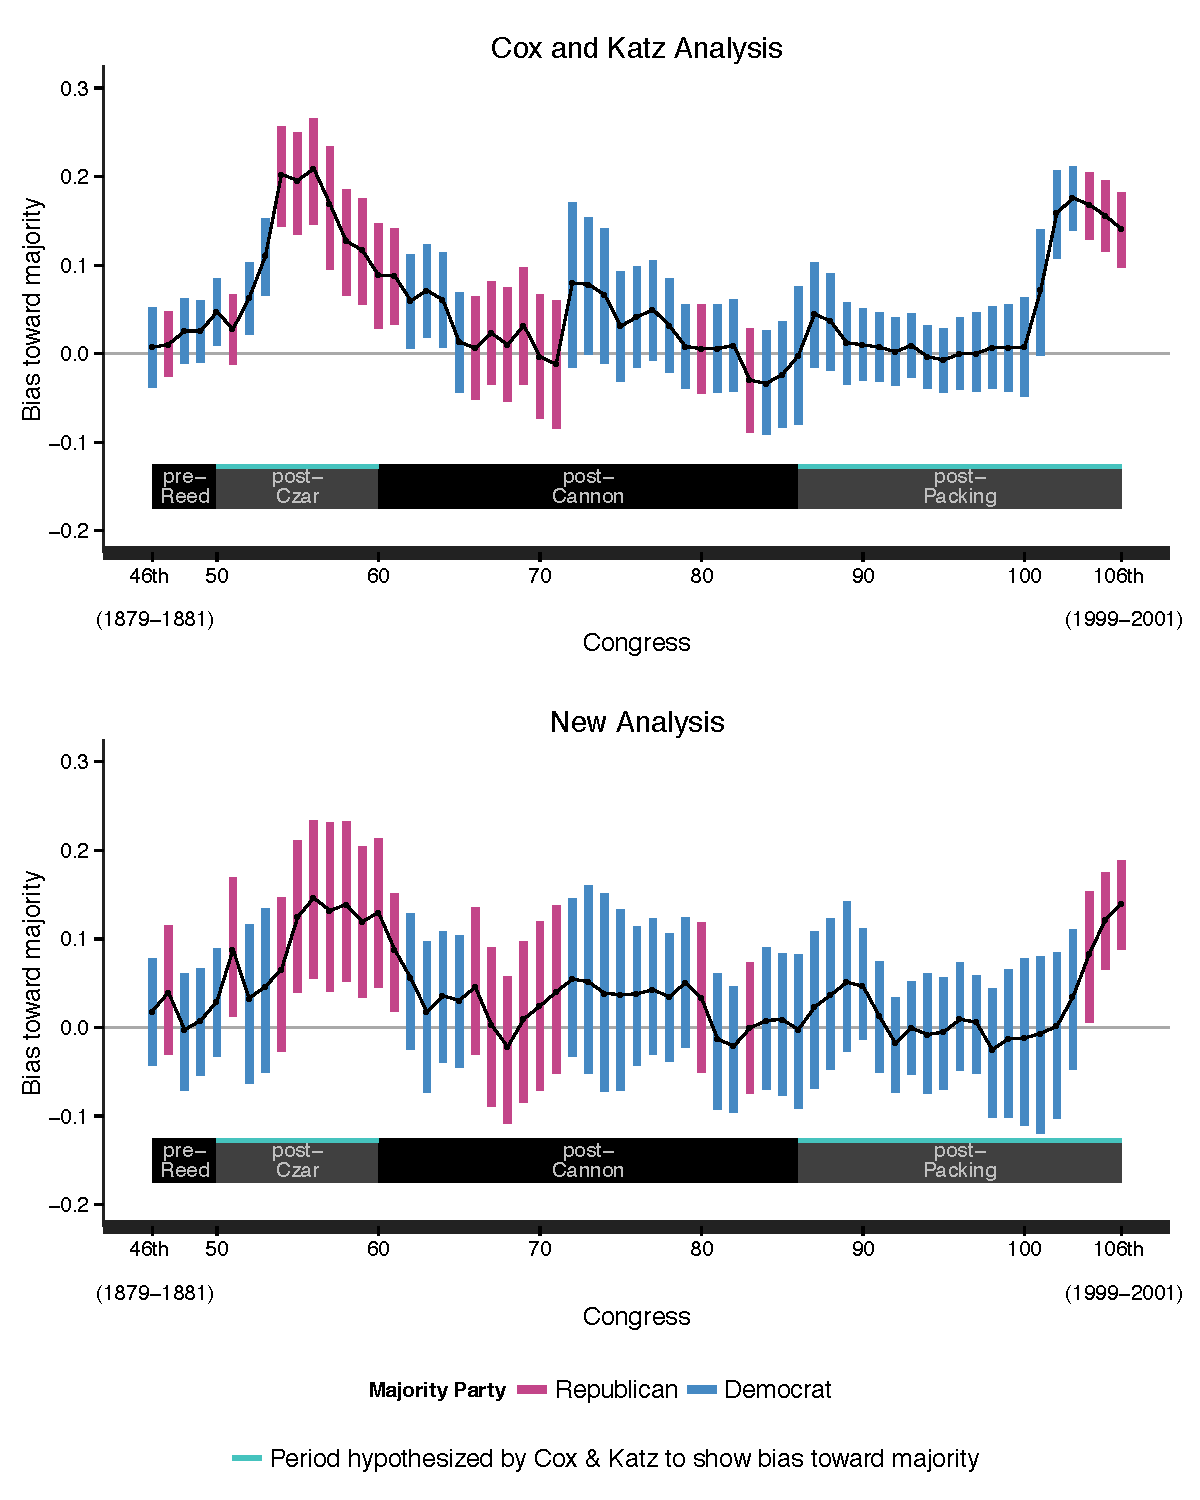
\includegraphics[scale=0.75]{sections/figs/ck_replication}
\caption{Estimated bias by Congress in Cox and Katz's analysis (top) and reanalysis (bottom). Vertical bars represent 95\%  intervals, with the black line connecting medians.}
\label{fig:ck_bias}
\end{figure}

Figure~\ref{fig:ck_bias} (page~\pageref{fig:ck_bias}) shows the estimates of bias towards the majority party over time from Cox and Katz's analysis and the reanalysis conducted here. Immediately noticeable is the fact that the new estimates have greater uncertainties, which is to be expected due to the potential for Cox and Katz's method to produce overly precise estimates, as discussed in \ref{subsection_methods}. Furthermore, while the new results provide some support for the hypothesis of bias during the post-Czar and post-Packing periods, the evidence is much weaker than that found by Cox and Katz. 


\subsection{Convergence diagnostics}
\label{subsection_convergence}

When inferences are made using posterior simulations generated by an MCMC algorithm it is essential to check for evidence of convergence to the target distribution. Although this process is not an exact science, there is no shortage of literature on the topic of monitoring convergence for MCMC and other iterative simulation algorithms. For this analysis, the recommendations in \citeA{gelman_handbook_2011} and \citeA{stan_development_team_stan_2015} are followed.\footnote{The various convergence diagnostics used here are introduced informally. More formal definitions and computational details can be found in \citeA{stan_development_team_stan_2015}, \citeA{gelman_handbook_2011}, and \citeA{gelman_bayesian_2013}.}

Six randomly initialized chains of 500 iterations (including 250 discarded warmup iterations) were simulated.\footnote{People new to HMC, NUTS, and Stan are often surprised by how few iterations are typically required, as it is not uncommon for Gibbs (and poorly tuned M-H) samplers to require hundreds of thousands of iterations to achieve convergence.} Figure~\ref{fig:ck_diagnostics} shows the distributions of three quantities calculated from the posterior sample. On the left is the distribution of the ratio of effective sample size to the number of iterations ($n_{\it eff}/N$). Roughly speaking, $n_{\it eff}$ is an estimate of the number of {\it independent} draws from the posterior distribution that would have the same expected variance as the the $N$ {\it dependent} draws actually obtained from the Markov chains. In this case $n_{\it eff}/N$ for all parameters is close to the ideal value of one, a reflection of Stan's efficiency. 

The distribution on the right in Figure~\ref{fig:ck_diagnostics} is the potential scale reduction statistic $\hat{R}$  \shortcite{gelman_rhat_1992}. The $\hat{R}$ statistic is a comparison of the variance of the simulations within individual chains to that of the simulations when chains are pooled. Here, the distribution of $\hat{R}$ shows that for all parameters the value is approximately one, indicating that little would be gained by running longer chains. 



\subsection{Model checking}
\label{subsection_model_checking}

\begin{figure}
\centering
	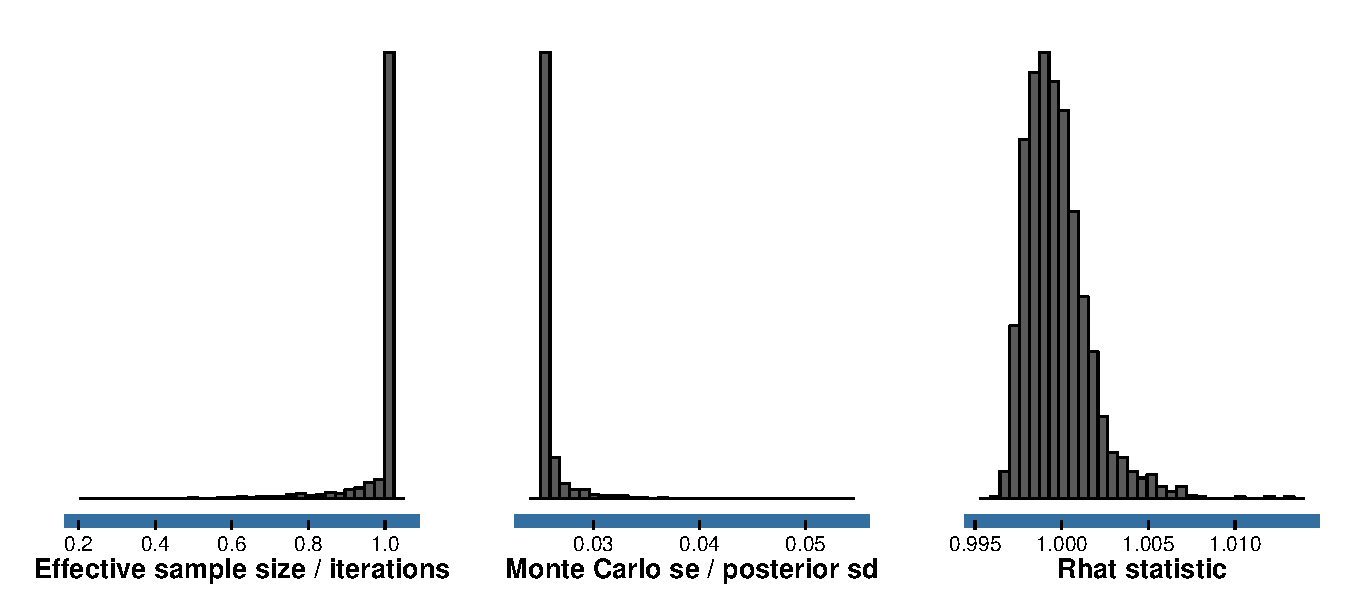
\includegraphics[scale=0.67]{sections/figs/ck_diagnostics}
\caption{Diagnostics}
\label{fig:ck_diagnostics}
\end{figure}



\begin{figure}
\centering
	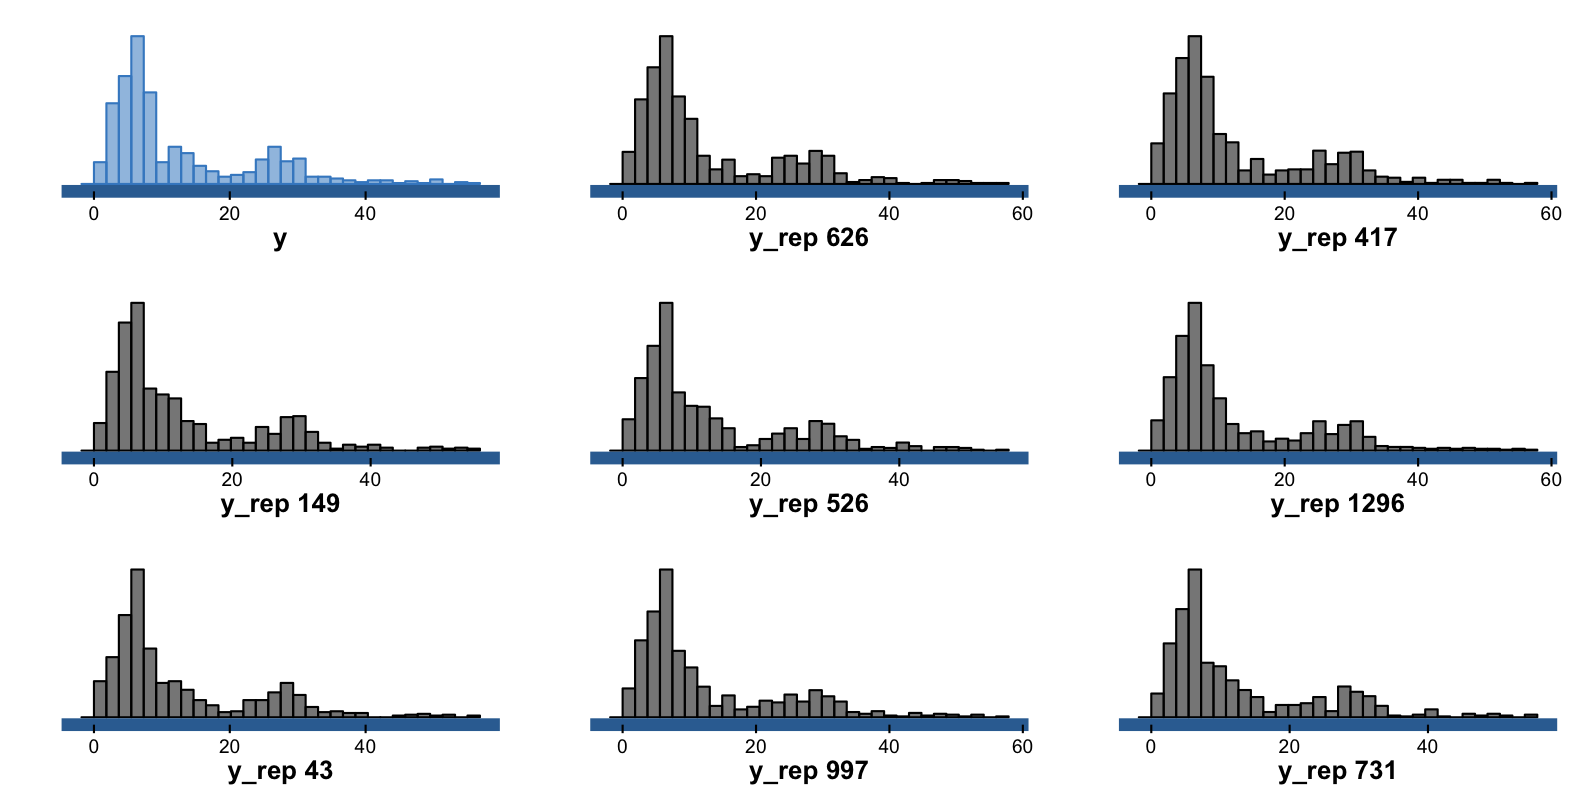
\includegraphics[scale=0.25]{sections/figs/ck_pp_hists}
\caption{Replications from posterior predictive distribution vs. observed data}
\label{fig:ck_pp_hists}
\end{figure}

\begin{figure}
\centering
	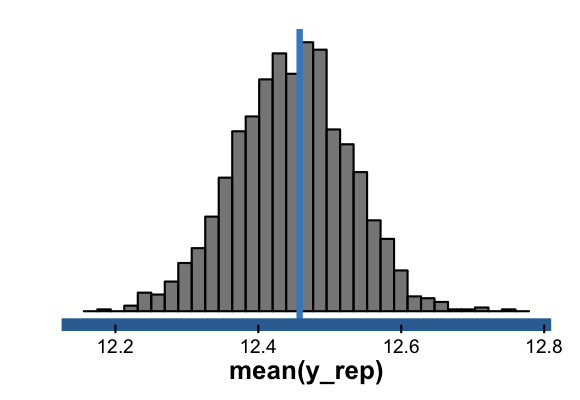
\includegraphics[scale=0.25]{sections/figs/ck_pp_test_statistics_mean}
	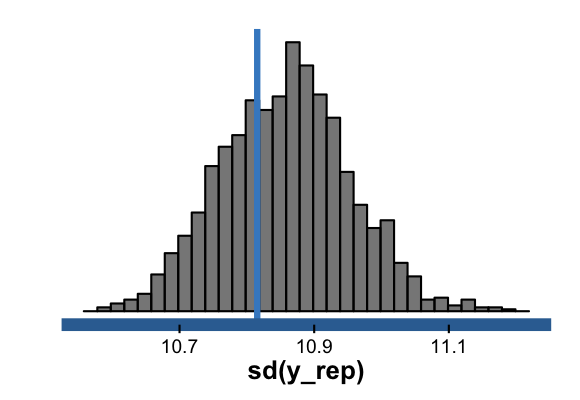
\includegraphics[scale=0.25]{sections/figs/ck_pp_test_statistics_sd}
\caption{Distributions of test statistics $T(y_{rep})$ vs observed values $T(y)$}
\label{fig:ck_pp_test_statistics}
\end{figure}

\begin{figure}
\centering
	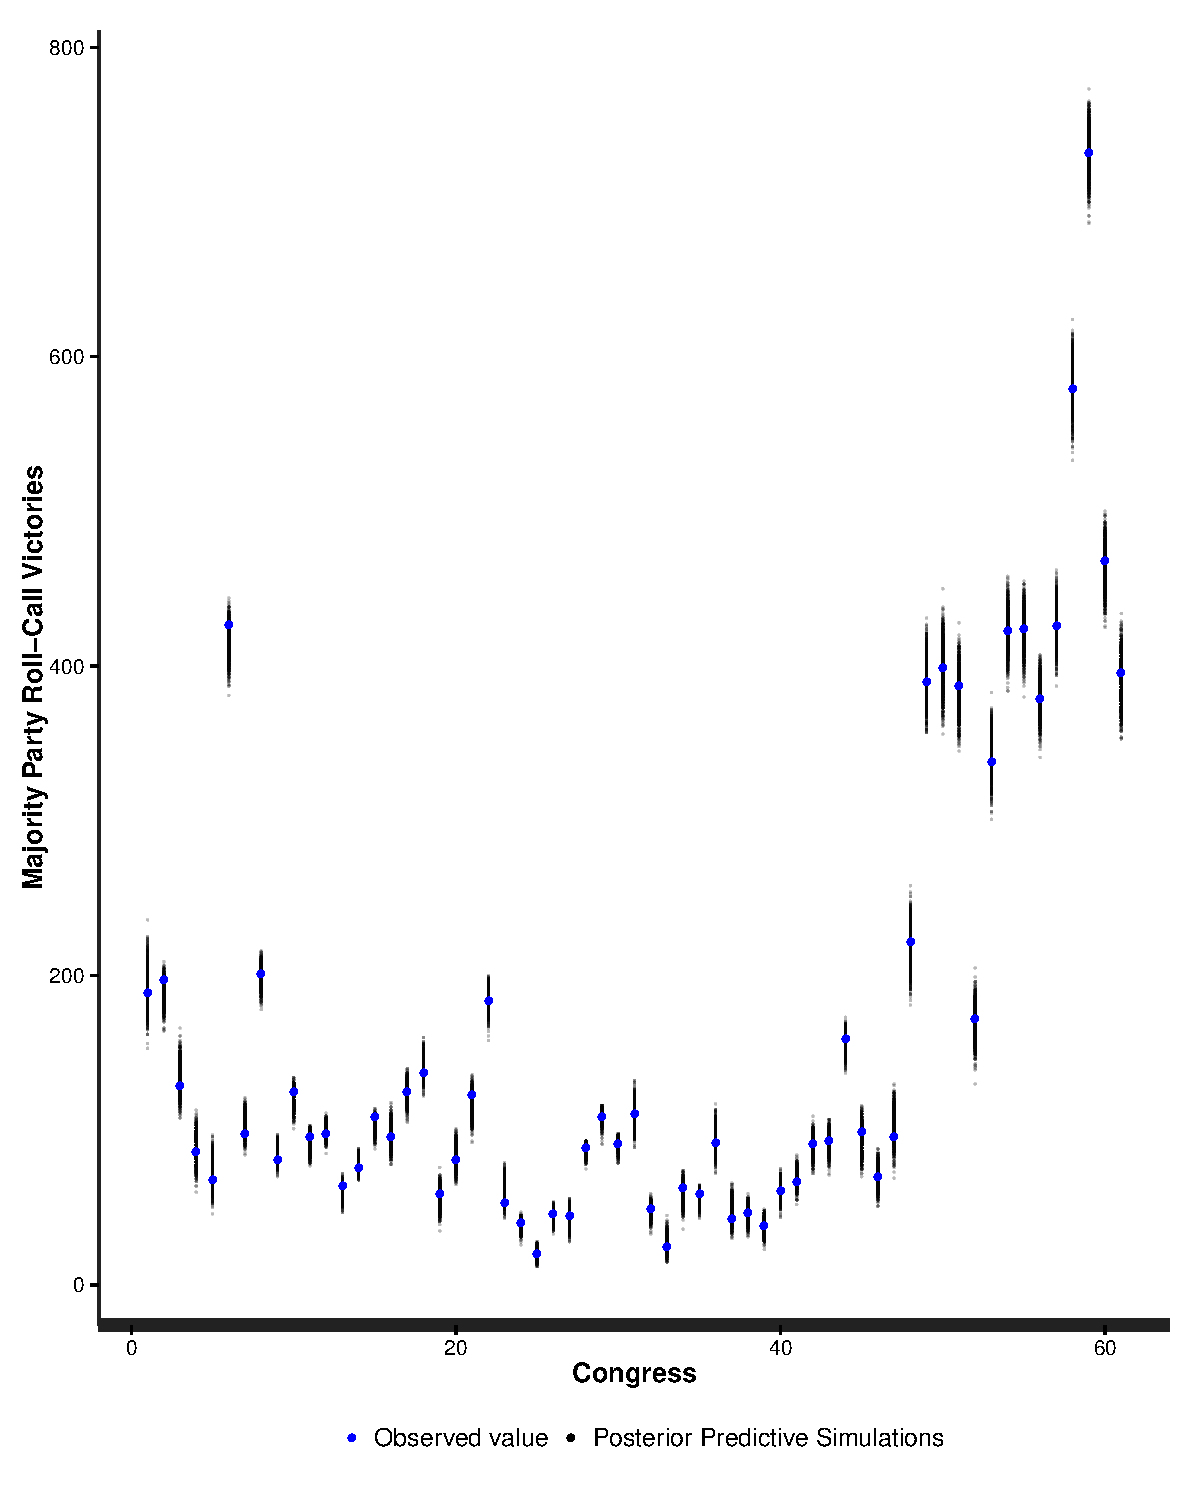
\includegraphics[scale=0.5]{sections/figs/ck_pp_nWins}
\caption{Replications from posterior predictive distribution vs. observed data}
\label{fig:ck_pp_nWins}
\end{figure}

